\documentclass[12pt]{article}
\usepackage{setspace}
\usepackage{float}
\usepackage{svg}
\usepackage{pdflscape}
\usepackage{longtable}
\usepackage{tikz}
\usepackage{amsmath}
\usepackage[scaled]{helvet}
\renewcommand\familydefault{\sfdefault}
\usepackage{caption}
\usepackage{subcaption}
\usepackage[hidelinks]{hyperref}
\usepackage[numbers]{natbib}
\usepackage[export]{adjustbox}
\hypersetup{ colorlinks, citecolor=black,
  filecolor=black,
  linkcolor=black,
  urlcolor=blue,
  pdftitle={Hardware Design and System Updates},
  pdfpagemode=FullScreen,
}
\usepackage{siunitx}
\usepackage{tabularx}
\usepackage{bookmark}
\bookmarksetup{
  numbered,
  open,
}
\newcommand\createfigurew[3]{
  \begin{center}
  \begin{figure}[H]
    \centering \includegraphics[width=\textwidth]{#1}
    \caption{#2}
    \label{#3}
  \end{figure}
  \end{center}
}
\newcommand\createfiguresw[4]{
  \begin{center}
  \begin{figure}[H]
    \centering \includegraphics[width=#1]{#2}
    \caption{#3}
    \label{#4}
  \end{figure}
  \end{center}
}
\newcommand\createfigurel[3]{
  \begin{center}
  \begin{figure}[H]
    \centering \includegraphics[height=0.8\textheight]{#1}
    \caption{#2}
    \label{#3}
  \end{figure}
  \end{center}
}
\newcommand\createfigurewsvg[3]{
 \begin{figure}[H]
  \begin{center}
    \centering\includesvg[width=\textwidth]{#1}
    \caption{#2}
    \label{#3}
  \end{center}
 \end{figure}
}
\usepackage{etoolbox}
\apptocmd{\thebibliography}{\raggedright}{}{}
\begin{document}
\linespread{1.0}
 \begin{titlepage}
  \begin{center}
    \large{University of Puerto Rico\\
    Mayagüez Campus\\
    \vspace{\baselineskip}
    Department of Electrical and Computer Engineering\\}
    \vspace{6cm}
    \Huge{\underline{Insulin Temperature Warning System}\\}
    \vspace{0.5\baselineskip}
    \large by\\
    Fabio J. Matos Nieves\\
    Enrique Chompré\\
    Guillermo Colón\\
    Rubén Marrero\\
    \vspace{3.5cm}
    For: Professor Manuel Jimenez\\
    Course: INEL 4217 Seccion 096\\
    Date: Febuary 2, 2023\\
    \normalsize

  \end{center}
\end{titlepage}

\linespread{2.0}
 \tableofcontents
 \listoffigures
 \listoftables
 \section{Completion Table}
\begin{table}[h]
 \begin{center}
  \begin{tabular}{|c|c|}
    \hline
    \multicolumn{2}{|c|}{Completion Table}\\
    \hline
    Module&Completion (\%)\\
    \hline
    Main Unit&20\%\\
    \hline
    Sub Unit&0\%\\
    \hline
    Power Supply (PSU)&80\%\\
    \hline
    Host Computer Software&0\%\\
    \hline
  \end{tabular}
 \end{center}
 \caption{Module Completion Table}
 \label{tab:comp-table}
\end{table}

 \section{Updated System Block Diagram}
\createfigurewsvg{../BDv4/Figures/bdv4-main.svg}{Main Unit System Architecture Block Diagram}{fig:bdv4-main}
\createfigurewsvg{../BDv4/Figures/bdv4-sub.svg}{Sub Unit System Architecture Block Diagram}{fig:bdv4-sub}

 \section{System Schematic Diagrams}
\begin{landscape}
  \begin{center}
  \begin{figure}[H]
    \centering \includegraphics[width=1.6\textwidth]{../Power-Supply/Main Unit PSU/main-unit-psu.png}
    \caption{Main Unit PSU Schematic}
    \label{fig:main-psu-schematic}
  \end{figure}
  \end{center}
\end{landscape}
\createfigurew{../Power-Supply/Sub Unit PSU/sub-unit-psu.png}{Sub Unit PSU Schematic}{fig:sub-psu-schematic}
\createfigurew{../Main-Unit/Figures/Main-Unit.png}{Main Unit Schematic}{fig:main-unit-schematic}
\createfigurew{../Sub-Unit/Figures/sub-unit.png}{Sub Unit Schematic}{fig:Sub-unit-schematic}
\begin{landscape}
  \begin{center}
  \begin{figure}[H]
    \centering 
\includegraphics[width=1.5\textwidth]{../Main-Unit-and-PSU/Figures/main-unit-and-psu.png}
    \caption{Main Unit with PSU Schematic}
    \label{fig:main-with-psu-schematic}
  \end{figure}
  \end{center}
\end{landscape}

 \begin{center}
\section{Bill of Materials}
\begin{landscape}
  \begin{table}[ht]
    \addtocounter{table}{-1}
  \begin{longtable}[c]{|c|c|c|c|c|c|c|c|c|}
    \hline
    \multicolumn{9}{|c|}{Bill of Materials: Main Unit}\\
    \hline
    Item\#&Qty&Description&Ref&Part\#&Unit Price&Est. Cost&Supplier&Datasheet\\
    \hline
    1&1&12V AC-DC Converter&U4&RAC03-12SK&\$7.70&\$7.70&\href{https://www.digikey.com/en/products/detail/recom-power/RAC03-12SK/10131801}{Digi-Key}&\href{https://recom-power.com/pdf/Powerline_AC-DC/RAC03-K.pdf}{Data-sheet}\\
    \hline
    2&1&Schottky Diode&CR1&1N5819&\$0.39&\$0.39&\href{https://www.digikey.com/en/products/detail/stmicroelectronics/1N5819/1037326}{Digi-key}&\href{https://www.st.com/content/ccc/resource/technical/document/datasheet/26/db/14/60/52/47/47/5b/CD00001625.pdf/files/CD00001625.pdf/jcr:content/translations/en.CD00001625.pdf}{Data-sheet}\\
    \hline
    3&2&Regular Diode&D1,D3&1N4004-G&\$0.21&\$0.42&\href{https://www.digikey.com/en/products/detail/comchip-technology/1N4004-G/1979655}{Digi-Key}&\href{https://www.comchiptech.com/admin/files/product/1N4001-G\%20Thru.\%201N4007-G\%20RevB.pdf}{Data-sheet}\\
    \hline
    4&2&3.6\si{\V} Battery&BT1,BT2&NURE18650-1&\$13.99&\$27.98&\href{https://www.batteriesplus.com/productdetails/nure18650=1}{BatteryPlus}&\href{https://www.batteriesplus.com/productdetails/nure18650=1}{Data-sheet}\\
    \hline
    5&2&3.3\si{\V} DC-DC Converter&DC1,DC2&K7803-500R3&\$3.25&\$6.50&\href{https://www.digikey.com/en/products/detail/recom-power/R-78E3-3-0-5/3593412?s=N4IgTCBcDaIEoFoDsAOAogZgHQYQBiwFYQBdAXyA}{Digi-Key}&\href{https://recom-power.com/pdf/Innoline/R-78E-0.5.pdf}{Data-sheet}\\
    \hline
    6&2&3.3\si{\V} LDO&U1-U2&BA33BC0T&\$2.62&\$5.24&\href{https://www.digikey.com/en/products/detail/rohm-semiconductor/BA33BC0T/722279?s=N4IgTCBcDaIEIEEDMS4GEAMAVEBdAvkA}{Digi-Key}&\href{https://www.rohm.com/datasheet?p=BA33BC0T&dist=Digi-key&media=referral&source=digi-key.com&campaign=Digi-key}{Data-sheet}\\
    \hline
    7&3&0.1\si{\micro\farad} 50\si{\V} Capacitor&C1,C2&UVR1H0R1MDD1TD&\$0.28&\$0.84&\href{https://www.digikey.com/en/products/detail/nichicon/UVR1H0R1MDD1TD/4328983}{Digi-Key}&\href{https://download.datasheets.com/pdfs/2016/10/6/6/6/44/578/nch_/manual/93896153625063e-uvr.pdf}{Data-sheet}\\
	\hline
    8&1&16 MHz MCU&U3&MSP430FR2110IPW16&\$1.21&\$1.21&\href{https://www.digikey.com/en/products/detail/texas-instruments/MSP430FR2110IPW16R/6570204}{Digi-key}&\href{https://www.ti.com/lit/ds/symlink/msp430fr2111.pdf?HQS=dis-dk-null-digikeymode-dsf-pf-null-wwe&ts=1678667024727&ref_url=https\%253A\%252F\%252Fgoogle.com}{Data-sheet}\\
     \hline
	9&1&Bluetooth Module& HM-10& HM-10& \$5.30&\$5.30&\href{https://www.amazon.com/HiLetgo-Bluetooth-Wireless-Compatible-Arduino/dp/B00WGPKZ8Y/ref=sr_1_3?crid=3SILST2625K4B&keywords=hm-10+ble+hiletgo&qid=1679932067&sprefix=hm-10+ble+hiletgo\%2Caps\%2C133&sr=8-3}{Amazon}&\href{https://people.ece.cornell.edu/land/courses/ece4760/PIC32/uart/HM10/DSD\%20TECH\%20HM-10\%20datasheet.pdf}{Data-sheet}\\
	\hline
    10&1&18650 Battery Holder&BT1,BT2&BK-18650-PC4&\$6.22&\$6.22&\href{https://www.digikey.com/en/products/detail/mpd-memory-protection-devices/BK-18650-PC4/2330513?s=N4IgTCBcDaIEIGkC0BGAHANgKwAYkAUBhAFhAF0BfIA}{Digi-Key}&\href{https://www.memoryprotectiondevices.com/datasheets/BK-18650-PC4-datasheet.pdf}{Data-sheet}\\
	\hline
    11&1&Op Amp&U4&MCP6022-I/P&\$1.97&\$1.97&\href{https://www.digikey.com/en/products/detail/microchip-technology/MCP6022-I-P/417828}{Digi-Key}&\href{https://ww1.microchip.com/downloads/en/DeviceDoc/20001685E.pdf}{Data-sheet}\\
	\hline
    12&1&39\si{\ohm} Resistor&R5&CF18JT39R0&\$0.10&\$0.10&\href{https://www.digikey.com/en/products/detail/stackpole-electronics-inc/CF18JT39R0/1741693?s=N4IgTCBcDaIMIDECMAOAUgFQMwE4BKADCALoC\%2BQA}{Digi-Key}&\href{https://www.seielect.com/Catalog/SEI-CF_CFM.pdf}{Data-sheet}\\
	\hline
    13&1&5.1\si{\ohm} Resistor&R6&CFM14JT5R10&\$0.10&\$0.10&\href{https://www.digikey.com/en/products/detail/stackpole-electronics-inc/CFM14JT5R10/1742230?s=N4IgTCBcDaIMIDECyBGALAKQCoFYBKKADCALoC\%2BQA}{Digi-Key}&\href{https://www.seielect.com/Catalog/SEI-CF_CFM.pdf}{Data-sheet}\\
	\hline
    14&1&1\si{\kilo\ohm} Resistor&R7&CF14JT1K00&\$0.10&\$0.10&\href{https://www.digikey.com/en/products/detail/stackpole-electronics-inc/CF14JT1K00/1741314}{Digi-Key}&\href{https://www.seielect.com/Catalog/SEI-CF_CFM.pdf}{Data-sheet}\\
	\hline
    15&1&620\si{\ohm} Resistor&R4&CF18JT620R&\$0.10&\$0.10&\href{https://www.digikey.com/en/products/detail/stackpole-electronics-inc/CF18JT620R/1741752?s=N4IgTCBcDaIMIDECMAOAUgFQGxgAwCUQBdAXyA}{Digi-Key}&\href{https://www.seielect.com/Catalog/SEI-CF_CFM.pdf}{Data-sheet}\\
	\hline
    16&1&5\si{\V} DC-DC Converter&DC4&TSR 1-2450&\$5.80&\$5.80&\href{https://www.digikey.com/en/products/detail/traco-power/TSR-1-2450/9383780}{Digi-Key}&\href{https://www.tracopower.com/sites/default/files/products/datasheets/tsr1_datasheet.pdf}{Data-sheet}\\
	\hline
    17&1&5\si{\V} LDO&U6&L7805CV&\$0.69&\$0.69&\href{https://www.digikey.com/en/products/detail/stmicroelectronics/L7805CV/585964}{Digi-Key}&\href{https://www.st.com/content/ccc/resource/technical/document/datasheet/41/4f/b3/b0/12/d4/47/88/CD00000444.pdf/files/CD00000444.pdf/jcr:content/translations/en.CD00000444.pdf}{Data-sheet}\\
	\hline
    18&1&Temperature Sensor&U5&TMP36GT9Z&\$2.40&\$2.40&\href{https://www.digikey.com/en/products/detail/analog-devices-inc/TMP36GT9Z/820404?s=N4IgTCBcDaICoFkAKBmAbAcTgTgFogF0BfIA}{Digi-Key}&\href{https://www.analog.com/media/en/technical-documentation/data-sheets/TMP35_36_37.pdf}{Data-sheet}\\
	\hline
    19&1&18650 Battery Charger&&Snado&\$12.69&\$12.69&\href{https://www.amazon.com/dp/B0721JP6FK?psc=1&ref=ppx_yo2ov_dt_b_product_details}{Amazon}&\href{https://www.amazon.com/dp/B0721JP6FK?psc=1&ref=ppx_yo2ov_dt_b_product_details}{Data-sheet}\\
	\hline
    20&2&330\si{\ohm} Resistor&R1,R2&CF18JT330R&\$0.10&\$0.20&\href{https://www.seielect.com/Catalog/SEI-CF_CFM.pdf}{Digi-Key}&\href{https://www.seielect.com/Catalog/SEI-CF_CFM.pdf}{Data-sheet}\\
	\hline
    21&1&100\si{\ohm} Resistor&R3&CF14JT100R&\$0.10&\$0.10&\href{https://www.digikey.com/en/products/detail/stackpole-electronics-inc/CF14JT100R/1741261}{Digi-Key}&\href{https://www.seielect.com/Catalog/SEI-CF_CFM.pdf}{Data-sheet}\\
	\hline
    22&1&Red LED&LED1&XLUR12D&\$0.29&\$0.29&\href{https://www.digikey.com/en/products/detail/sunled/XLUR12D/4745846}{Digi-Key}&\href{https://octopart.com/datasheet/lhg3392-jameco+valuepro-2312745}{Data-sheet}\\
	\hline
    23&1&Green LED&LED2&WP7113GD&\$0.33&\$0.33&\href{https://www.digikey.com/en/products/detail/kingbright/WP7113GD/1747662}{Digi-Key}&\href{https://octopart.com/datasheet/lhg3392-jameco+valuepro-2312745}{Data-sheet}\\
	\hline
    \multicolumn{5}{|c|}{}&Total&\$98.66&\multicolumn{2}{c|}{}\\
    \hline
  \end{longtable}
  \caption{Bill of Materials: Main Unit}
  \label{BOM:Main-Unit}
  \end{table}
\begin{table}[ht]
    \addtocounter{table}{-1}
  \begin{longtable}[c]{|c|c|c|c|c|c|c|c|c|}
    \hline
    \multicolumn{9}{|c|}{Bill of Materials: Sub Unit}\\
    \hline
    Item\#&Qty&Description&Ref&Part\#&Unit Price&Est. Cost&Supplier&Datasheet\\
    \hline
    1&2&3.6\si{\V} Battery&BT1,BT2&NURE18650-1&\$13.99&\$27.98&\href{https://www.batteriesplus.com/productdetails/nure18650=1}{BatteryPlus}&\href{https://www.batteriesplus.com/productdetails/nure18650=1}{Data-sheet}\\
    \hline
    2&1&3.3\si{\V} DC-DC Converter&DC1&K7803-500R3&\$2.26&\$2.26&\href{https://www.digikey.com/en/products/detail/mornsun-america-llc/K7803-500R3/13168320}{Digi-Key}&\href{https://www.mornsun-power.com/html/pdf/K7803-500R3.html}{Data-sheet}\\
    \hline
    3&1&3.3\si{\V} LDO&U1&BA033CC0FP-E2&\$1.41&\$1.41&\href{https://www.digikey.com/en/products/detail/rohm-semiconductor/BA033CC0FP-E2/722186?s=N4IgTCBcDaIEIEEAMBmFBhdSBiAFAtAKIQC6AvkA}{Digi-Key}&\href{https://www.rohm.com/datasheet?p=BA033CC0FP&dist=Digi-key&media=referral&source=digi-key.com&campaign=Digi-key}{Data-sheet}\\
    \hline
    4&1&0.1\si{\micro\farad} 50\si{\V} Capacitor&C1,C2&UVR1H0R1MDD1TD&\$0.28&\$0.28&\href{https://www.digikey.com/en/products/detail/nichicon/UVR1H0R1MDD1TD/4328983}{Digi-Key}&\href{https://download.datasheets.com/pdfs/2016/10/6/6/6/44/578/nch_/manual/93896153625063e-uvr.pdf}{Data-sheet}\\
    \hline
    5&1&16\si{\MHz} MCU&U2&MSP430FR2000IPW16&\$1.31&\$1.31&\href{https://www.digikey.com/en/products/detail/texas-instruments/MSP430FR2000IPW16/7650247}{Digi-Key}&\href{https://www.ti.com/general/docs/suppproductinfo.tsp?distId=10&gotoUrl=https\%3A\%2F\%2Fwww.ti.com\%2Flit\%2Fgpn\%2Fmsp430fr2000}{Data-Sheet}\\
    \hline
    6&1&68\si{\ohm} Resistor&R1&CF18JT68R0&\$0.10&\$0.10&\href{https://www.digikey.com/en/products/detail/stackpole-electronics-inc/CF18JT68R0/1741755}{Digi-Key}&\href{https://www.seielect.com/Catalog/SEI-CF_CFM.pdf}{Data-sheet}\\
    \hline
    7&1&Red LED&LED1&SSL-LX3052ID&\$0.46&\$0.46&\href{https://www.digikey.com/en/products/detail/lumex-opto-components-inc/SSL-LX3052ID/39603?s=N4IgTCBcDaIMpwDIFpEA0DMAGArGAkgCIgC6AvkA}{Digi-Key}&\href{https://www.lumex.com/spec/SSL-LX3052ID.pdf}{Data-sheet}\\
	\hline
    8&1&5\si{\V} DC-DC Converter&DC2&TSR 1-2450&\$5.80&\$5.80&\href{https://www.digikey.com/en/products/detail/traco-power/TSR-1-2450/9383780}{Digi-Key}&\href{https://www.tracopower.com/sites/default/files/products/datasheets/tsr1_datasheet.pdf}{Data-sheet}\\
	\hline
    9&1&5\si{\V} LDO&U5&L7805CV&\$0.69&\$0.69&\href{https://www.digikey.com/en/products/detail/stmicroelectronics/L7805CV/585964}{Digi-Key}&\href{https://www.st.com/content/ccc/resource/technical/document/datasheet/41/4f/b3/b0/12/d4/47/88/CD00000444.pdf/files/CD00000444.pdf/jcr:content/translations/en.CD00000444.pdf}{Data-sheet}\\
    \hline
	10&1&Bluetooth Module& HM-10& HM-10& \$5.30&\$5.30&\href{https://www.amazon.com/HiLetgo-Bluetooth-Wireless-Compatible-Arduino/dp/B00WGPKZ8Y/ref=sr_1_3?crid=3SILST2625K4B&keywords=hm-10+ble+hiletgo&qid=1679932067&sprefix=hm-10+ble+hiletgo\%2Caps\%2C133&sr=8-3}{Amazon}&\href{https://people.ece.cornell.edu/land/courses/ece4760/PIC32/uart/HM10/DSD\%20TECH\%20HM-10\%20datasheet.pdf}{Data-sheet}\\
    \hline
    11&1&18650 Battery Holder&BT1,BT2&BK-18650-PC4&\$6.22&\$6.22&\href{https://www.digikey.com/en/products/detail/mpd-memory-protection-devices/BK-18650-PC4/2330513?s=N4IgTCBcDaIEIGkC0BGAHANgKwAYkAUBhAFhAF0BfIA}{Digi-Key}&\href{https://www.memoryprotectiondevices.com/datasheets/BK-18650-PC4-datasheet.pdf}{Data-sheet}\\
    \hline
    12&1&Op Amp&U3&TLR342F-GE2&\$0.70&\$0.70&\href{https://www.digikey.com/en/products/detail/rohm-semiconductor/TLR342F-GE2/7896247?s=N4IgTCBcDaICoBkBKBmALGAYgWgOIFEIBdAXyA}{Digi-Key}&\href{https://www.rohm.com/datasheet?p=TLR342F&dist=Digi-key&media=referral&source=digi-key.com&campaign=Digi-key}{Data-sheet}\\
	\hline
    13&1&39\si{\ohm} Resistor&R6&CF18JT39R0&\$0.10&\$0.10&\href{https://www.digikey.com/en/products/detail/stackpole-electronics-inc/CF18JT39R0/1741693?s=N4IgTCBcDaIMIDECMAOAUgFQMwE4BKADCALoC\%2BQA}{Digi-Key}&\href{https://www.seielect.com/Catalog/SEI-CF_CFM.pdf}{Data-sheet}\\
	\hline
    14&1&5.1\si{\ohm} Resistor&R7&CFM14JT5R10&\$0.10&\$0.10&\href{https://www.digikey.com/en/products/detail/stackpole-electronics-inc/CFM14JT5R10/1742230?s=N4IgTCBcDaIMIDECyBGALAKQCoFYBKKADCALoC\%2BQA}{Digi-Key}&\href{https://www.seielect.com/Catalog/SEI-CF_CFM.pdf}{Data-sheet}\\
	\hline
    15&1&1\si{\kilo\ohm} Resistor&R8&CF14JT1K00&\$0.10&\$0.10&\href{https://www.digikey.com/en/products/detail/stackpole-electronics-inc/CF14JT1K00/1741314}{Digi-Key}&\href{https://www.seielect.com/Catalog/SEI-CF_CFM.pdf}{Data-sheet}\\
	\hline
    16&1&620\si{\ohm} Resistor&R5&CF18JT620R&\$0.10&\$0.10&\href{https://www.digikey.com/en/products/detail/stackpole-electronics-inc/CF18JT620R/1741752?s=N4IgTCBcDaIMIDECMAOAUgFQGxgAwCUQBdAXyA}{Digi-Key}&\href{https://www.seielect.com/Catalog/SEI-CF_CFM.pdf}{Data-sheet}\\
	\hline
    17&1&Temperature Sensor&U4&TMP36GT9Z&\$2.40&\$2.40&\href{https://www.digikey.com/en/products/detail/analog-devices-inc/TMP36GT9Z/820404?s=N4IgTCBcDaICoFkAKBmAbAcTgTgFogF0BfIA}{Digi-Key}&\href{https://www.analog.com/media/en/technical-documentation/data-sheets/TMP35_36_37.pdf}{Data-sheet}\\
	\hline
    18&1&18650 Battery Charger&&Snado&\$12.69&\$12.69&\href{https://www.amazon.com/dp/B0721JP6FK?psc=1&ref=ppx_yo2ov_dt_b_product_details}{Amazon}&\href{https://www.amazon.com/dp/B0721JP6FK?psc=1&ref=ppx_yo2ov_dt_b_product_details}{Data-sheet}\\
	\hline
    \multicolumn{5}{|c|}{}&Total&\$74.49&\multicolumn{2}{c|}{}\\
    \hline
  \end{longtable}
  \caption{Bill of Materials: Sub Unit}
  \label{BOM:Sub-Unit}
  \end{table}
\end{landscape}
  \end{center}

 \section{Power, Voltage Compatibility and Timing Analysis}
\subsection{Main Unit PSU}
According to the RAC03-12SK data sheet\cite{RAC0312SK}, the AC/DC converter can handle from 85\si{\V}AC to 264\si{\V}AC and produce 12\si{\V}DC at its output. Since this design will be tested in a 120\si{\V}AC electrical system, it is compatible.\\ At the output of the AC/DC converter, a 1N4004-G diode\cite{1N4004G} and a R78-E3.3-0.5 3.3\si{\V} DC/DC converter\cite{R78E330} (DC2) are placed in parallel. For DC2, according to its data sheet, is compatible within a voltage range of 6\si{\V} to 28\si{\V}. Since DC2 is at the output of the 12\si{\V} AC/DC converter, it is compatible.\\ At the node at the right of D1 (N\$5), when mains power is available is calculated as follows:
\begin{equation}
  V_{N\$5} = 12 -  V_{D}
  \label{eq:mains-batt-node-eqation-mains-available}
\end{equation}
where $V_{D}$ is the diode drop of the 1N4004-G which according to its data sheet is 1.1\si{\V}, resulting in $N\$5$ equal to 10.9\si{\V}. When there is mains power available, the node will be at 10.9\si{\V}, the batteries will be trying to conduct but since the voltage of the two 3.6\si{\V} cells in series will be 7.2\si{\V}, minus the diode drop of CR1\cite{1N5819} will be $7.2 - 0.55 = 6.65\si{\V}$. Therefore, the potential difference between mains power and battery power is $-4.25\si{\V}$, therefore CR1 will be placed in reverse bias and thus the batteries will not conduct, but since the negative potential difference is low, it is compatible, according to the 1N5819 data sheet\cite{1N5819}.\\ When mains power is available DC1, another K7803-500R3, will receive a voltage of 10.9\si{\V} and as mentioned above is compatible and will produce a 3.3\si{\V} output. At the outputs of both DC1,DC2 there are identical 3.3\si{\V} LDOs (BA33BC0T)\cite{BA33BC0T}, which according to their data sheet can accept up to 16\si{\V} which is compatible since U1 and U2 are being supplied by 3.3\si{\V} DC/DC converters and thus are compatible. At the outputs of U1 and U2 are C2 and C3 respectively, that are 0.1\si{\micro\farad} filtering capacitors whose voltage rating is 50\si{\V} which are compatible.\\ Going back to $N\$5$ DC4 (5\si{\V} DC/DC converter) is in parallel with DC1, thus when there is mains power available, will be supplied 10.9\si{\V}. According to the TSR 1-2450 (DC4) data sheet\cite{TSR12450} it can accept a DC voltage from 6.5\si{\V} to 36\si{\V} thus making it compatible and will output 5\si{\V} DC. At the output of DC4, a 5\si{\V} LDO is fed (L7805CV
), whose data sheet\cite{L7805CV} says that it can handle up to 36\si{\V} thus making it compatible since the output of DC4 is 5\si{\V}. Similarly to C3 and C4, a 0.1\si{\micro\farad} capacitor is placed in parallel with the output and is compatible since it has the same voltage rating of 50\si{\V}.\\ When mains power is not available DC2 will shutdown and D1 will be placed in reverse bias since CR1 will be conducting due to $N\$5$ will be at 0\si{\V} when mains power is not available and then will be placed at 6.65\si{\V}. Since DC1, DC2 and DC4 all have a minimum voltage less than 6.65\si{\V} they are all compatible and the LDOs and capacitors will operate as normal.
\subsection{Sub Unit PSU}
\subsection{Main Unit}
\subsection{Sub Unit}

 \section{Individual Block Diagrams, Schematics and Pictures}
\subsection{Main Unit}
\subsubsection{Block Diagrams}
\createfigurewsvg{../Individual-BD-SCH-Pictures/Figures/main-unit.svg}{Main Unit Architectural Block Diagram}{fig:main-bd-indv}
\subsubsection{Schematics}
\begin{landscape}
  \begin{center}
  \begin{figure}[H]
    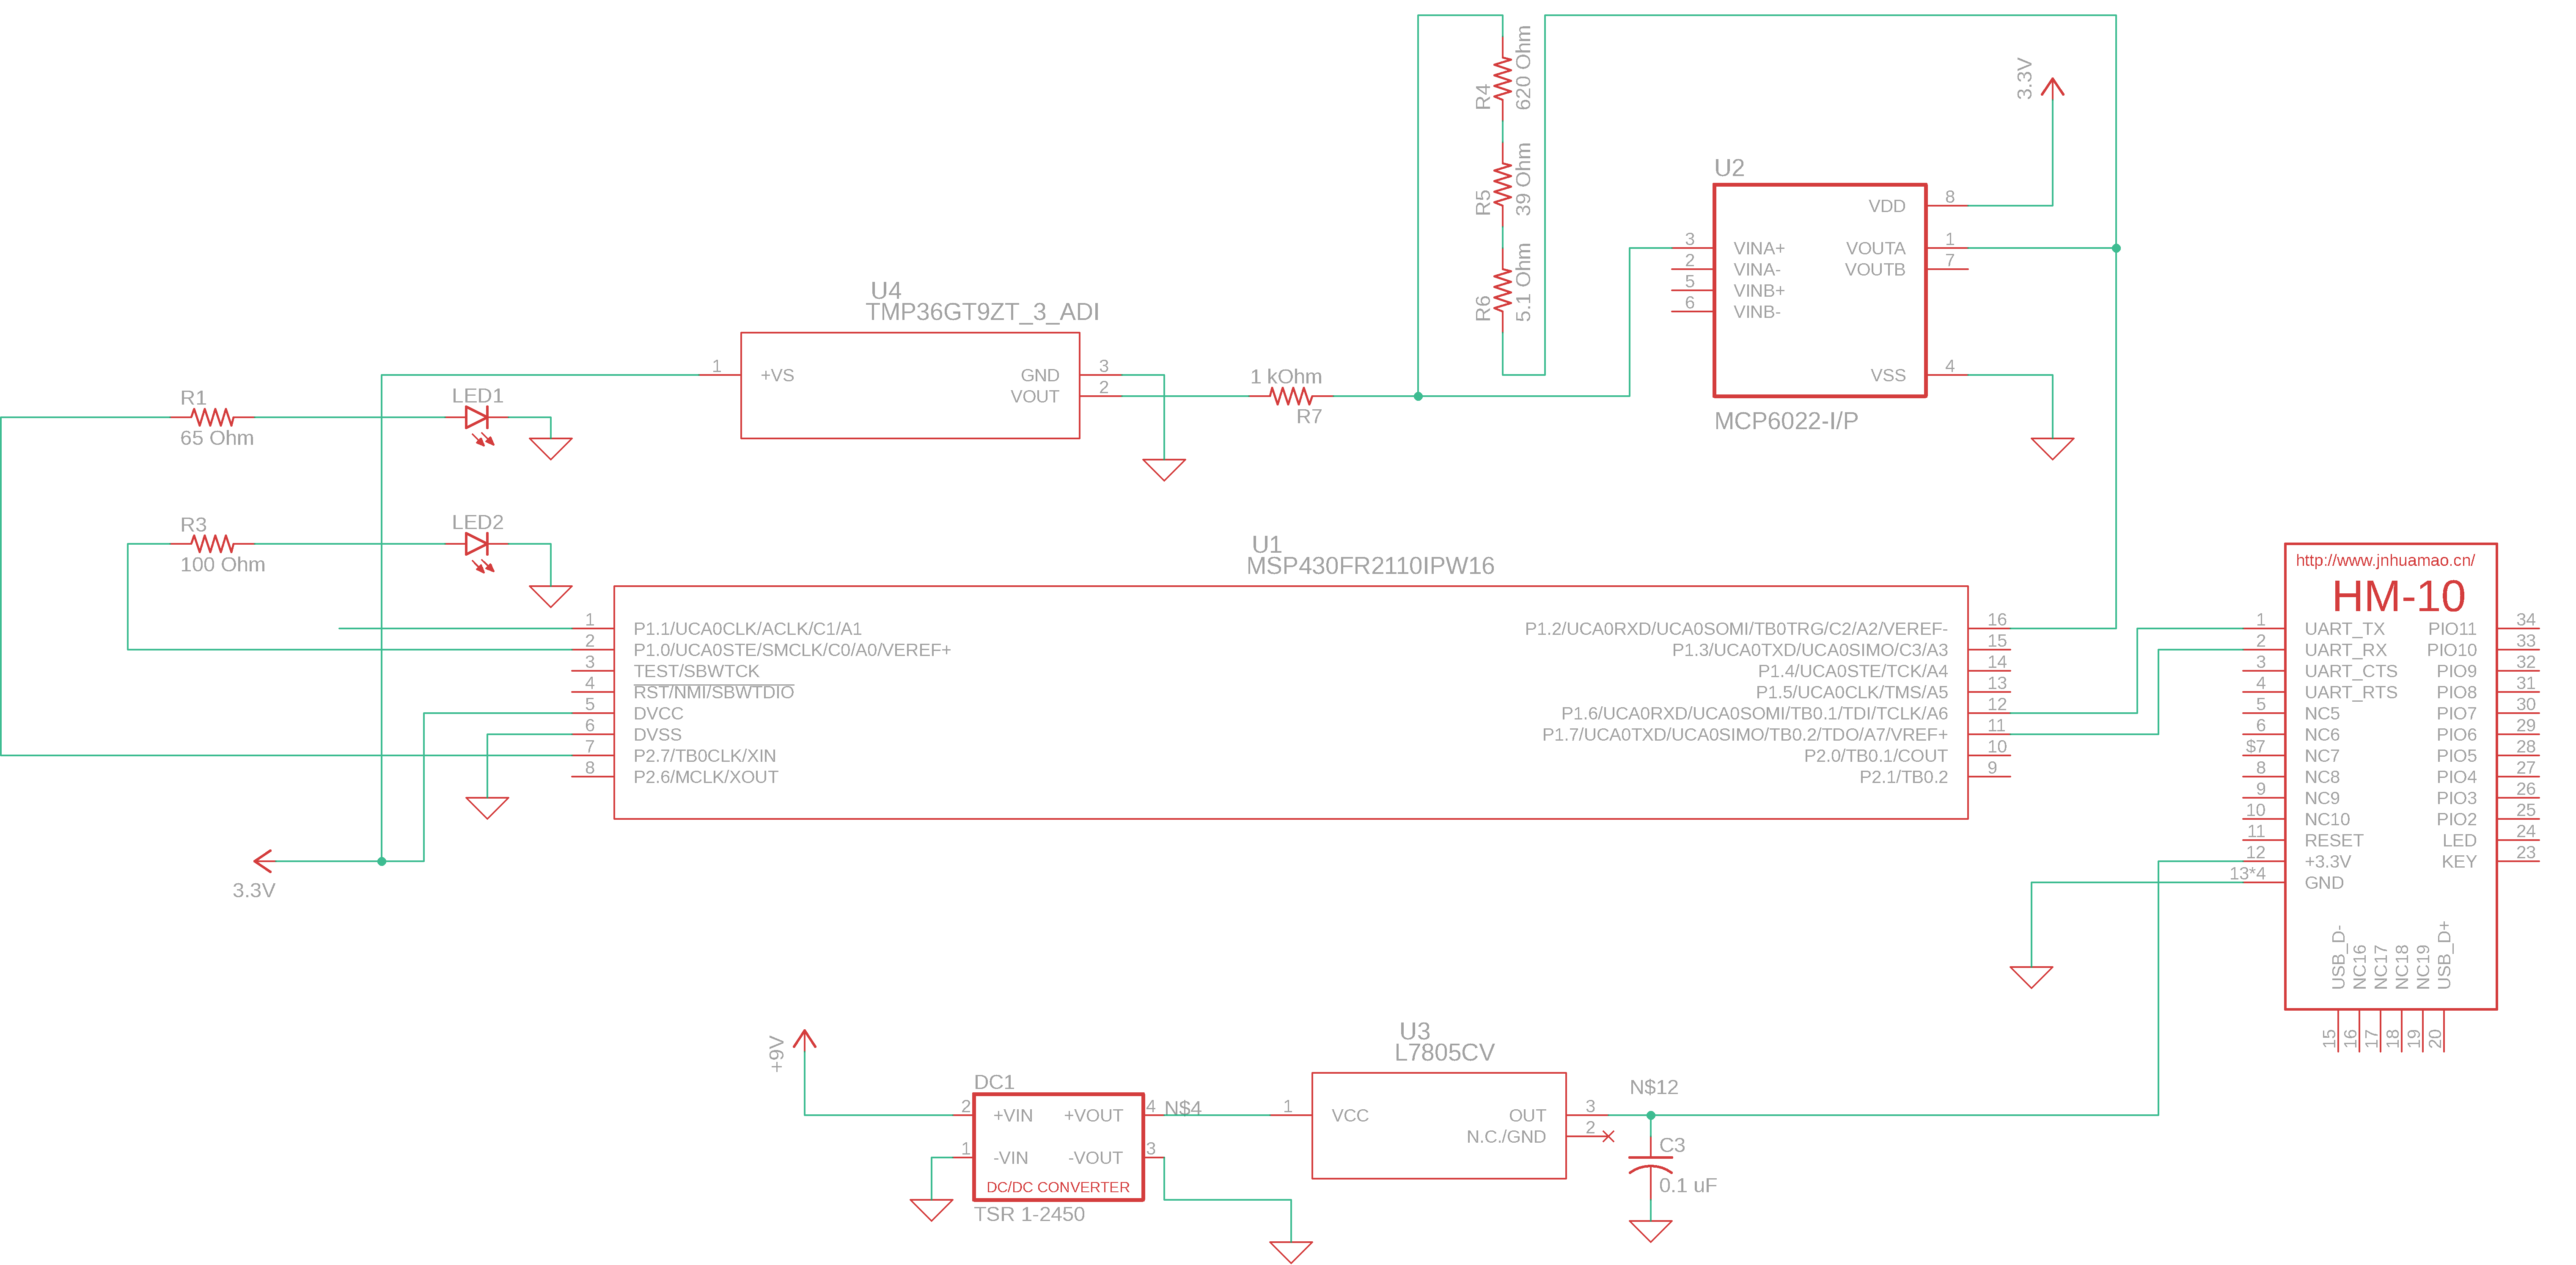
\includegraphics[width=\pdfpagewidth,height=0.75\textheight]{../System-Schematic-Diagrams/Figures/Main-Unit.png}
    \caption{Main Unit Schematic}
    \label{fig:main-unit-schematic}
  \end{figure}
  \end{center}
\end{landscape}
\subsubsection{Pictures}
\createfigurew{../Individual-BD-SCH-Pictures/Figures/main-unit-pic-1.jpeg}{Main unit Picture 1}{fig:main-unit-pic-1}
\createfigurew{../Individual-BD-SCH-Pictures/Figures/main-unit-pic-2.jpeg}{Main unit Picture 2}{fig:main-unit-pic-2}
\createfigurew{../Individual-BD-SCH-Pictures/Figures/main-unit-pic-3.jpeg}{Main unit Picture 3}{fig:main-unit-pic-3}
\createfigurew{../Individual-BD-SCH-Pictures/Figures/main-unit-pic-4.jpeg}{Main unit Picture 4}{fig:main-unit-pic-4}
\subsection{Sub Unit}
\subsubsection{Block Diagrams}
\createfigurewsvg{../Individual-BD-SCH-Pictures/Figures/sub-unit.svg}{Sub Unit Architectural Block Diagram}{fig:sub-bd-indv}
\subsubsection{Schematics}
\begin{landscape}
  \begin{center}
  \begin{figure}[H]
    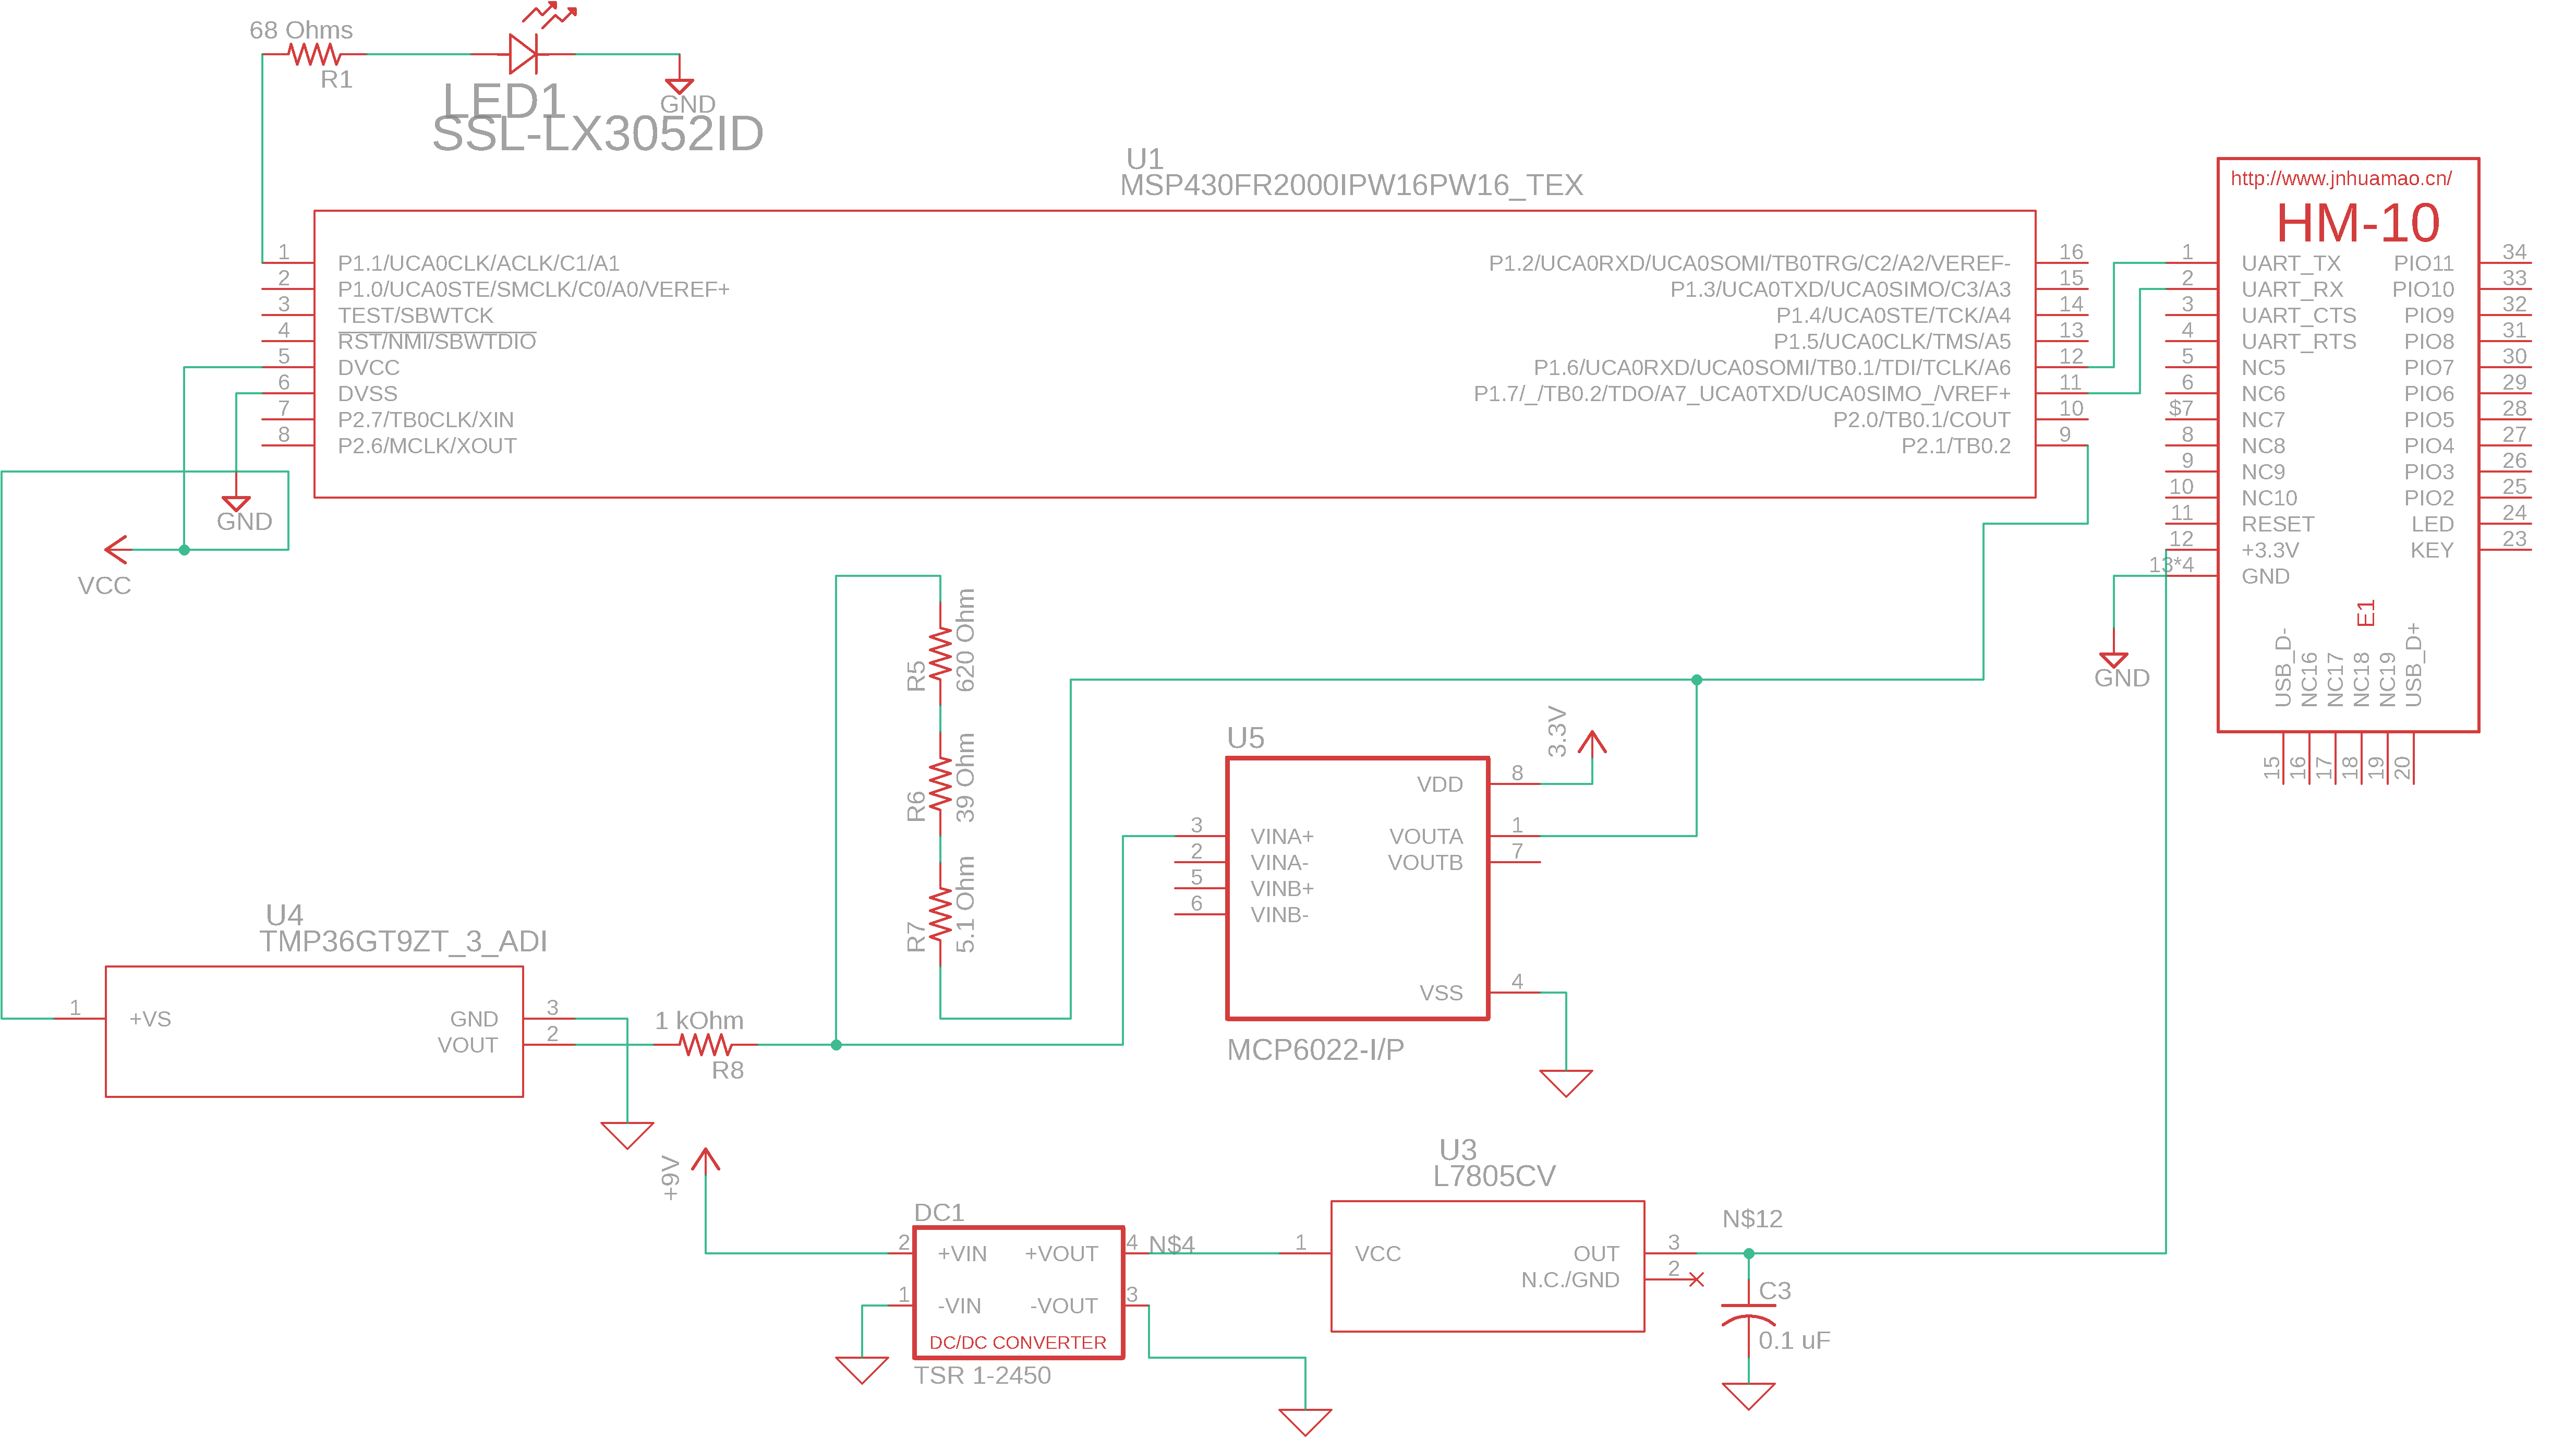
\includegraphics[width=\pdfpagewidth,height=0.70\textheight]{../System-Schematic-Diagrams/Figures/sub-unit.png}
    \caption{Sub Unit Schematic}
    \label{fig:sub-unit-schematic}
  \end{figure}
  \end{center}
\end{landscape}
\subsubsection{Pictures}
  \subsection{Power Supply}
\subsubsection{Block Diagrams}
\createfigurewsvg{../Individual-BD-SCH-Pictures/Figures/main-unit-psu.svg}{Main Unit PSU Architectural Block Diagram}{fig:main-psu-bd-indv}
\createfigurewsvg{../Individual-BD-SCH-Pictures/Figures/sub-unit-psu.svg}{Sub Unit PSU Architectural Block Diagram}{fig:sub-psu-bd-indv}
\subsubsection{Schematics}
\begin{landscape}
  \begin{center}
  \begin{figure}[H]
    \includegraphics[width=1.6\textwidth, left]{../System-Schematic-Diagrams/Figures/main-unit-psu.png}
    \caption{Main Unit PSU Schematic}
    \label{fig:main-psu-schematic}
  \end{figure}
  \end{center}
\createfigurew{../System-Schematic-Diagrams/Figures/sub-unit-psu.png}{Sub Unit PSU Schematic}{fig:sub-psu-schematic}
\end{landscape}
\subsubsection{Pictures}
\createfigurew{../Individual-BD-SCH-Pictures/Figures/main-unit-3.3V-1.jpeg}{Main unit PSU 3.3V Output Picture 1}{fig:main-unit-psu-1}
\createfigurew{../Individual-BD-SCH-Pictures/Figures/main-unit-3.3V-1.jpeg}{Main unit PSU 3.3V Output Picture 2}{fig:main-unit-psu-2}
\createfigurew{../Individual-BD-SCH-Pictures/Figures/main-unit-3.3V-1.jpeg}{Main unit PSU 4V Output Picture}{fig:main-unit-psu-3}
\createfigurew{../Individual-BD-SCH-Pictures/Figures/sub-unit-3.3V.jpeg}{Sub unit PSU 3.3V Output Picture}{fig:sub-unit-psu-1}
\createfigurew{../Individual-BD-SCH-Pictures/Figures/sub-unit-4V.jpeg}{Sub unit PSU 4V Output Picture}{fig:sub-unit-psu-2}

 \section{Detailed Software Plan Per Module}

 \bibliographystyle{IEEEtranN}
\bibliography{../References/references.bib}

\end{document}
